\chapter{Robot Organization}\label{ch:robot_organization}

\section{Network Configuration}\label{sec:network_configuration}
Each robot has its own local area network (LAN) that facilitates connectivity of components and computation. 

Not all components are hardwired to the network; some must be connected to a PC via USB.
As such, the components connected directly to a PC are local to that PC and can only be brought up on that PC. See Figure \ref{fig:network_map} for details on the connectivity of the system.


\begin{figure}[h]
\centering
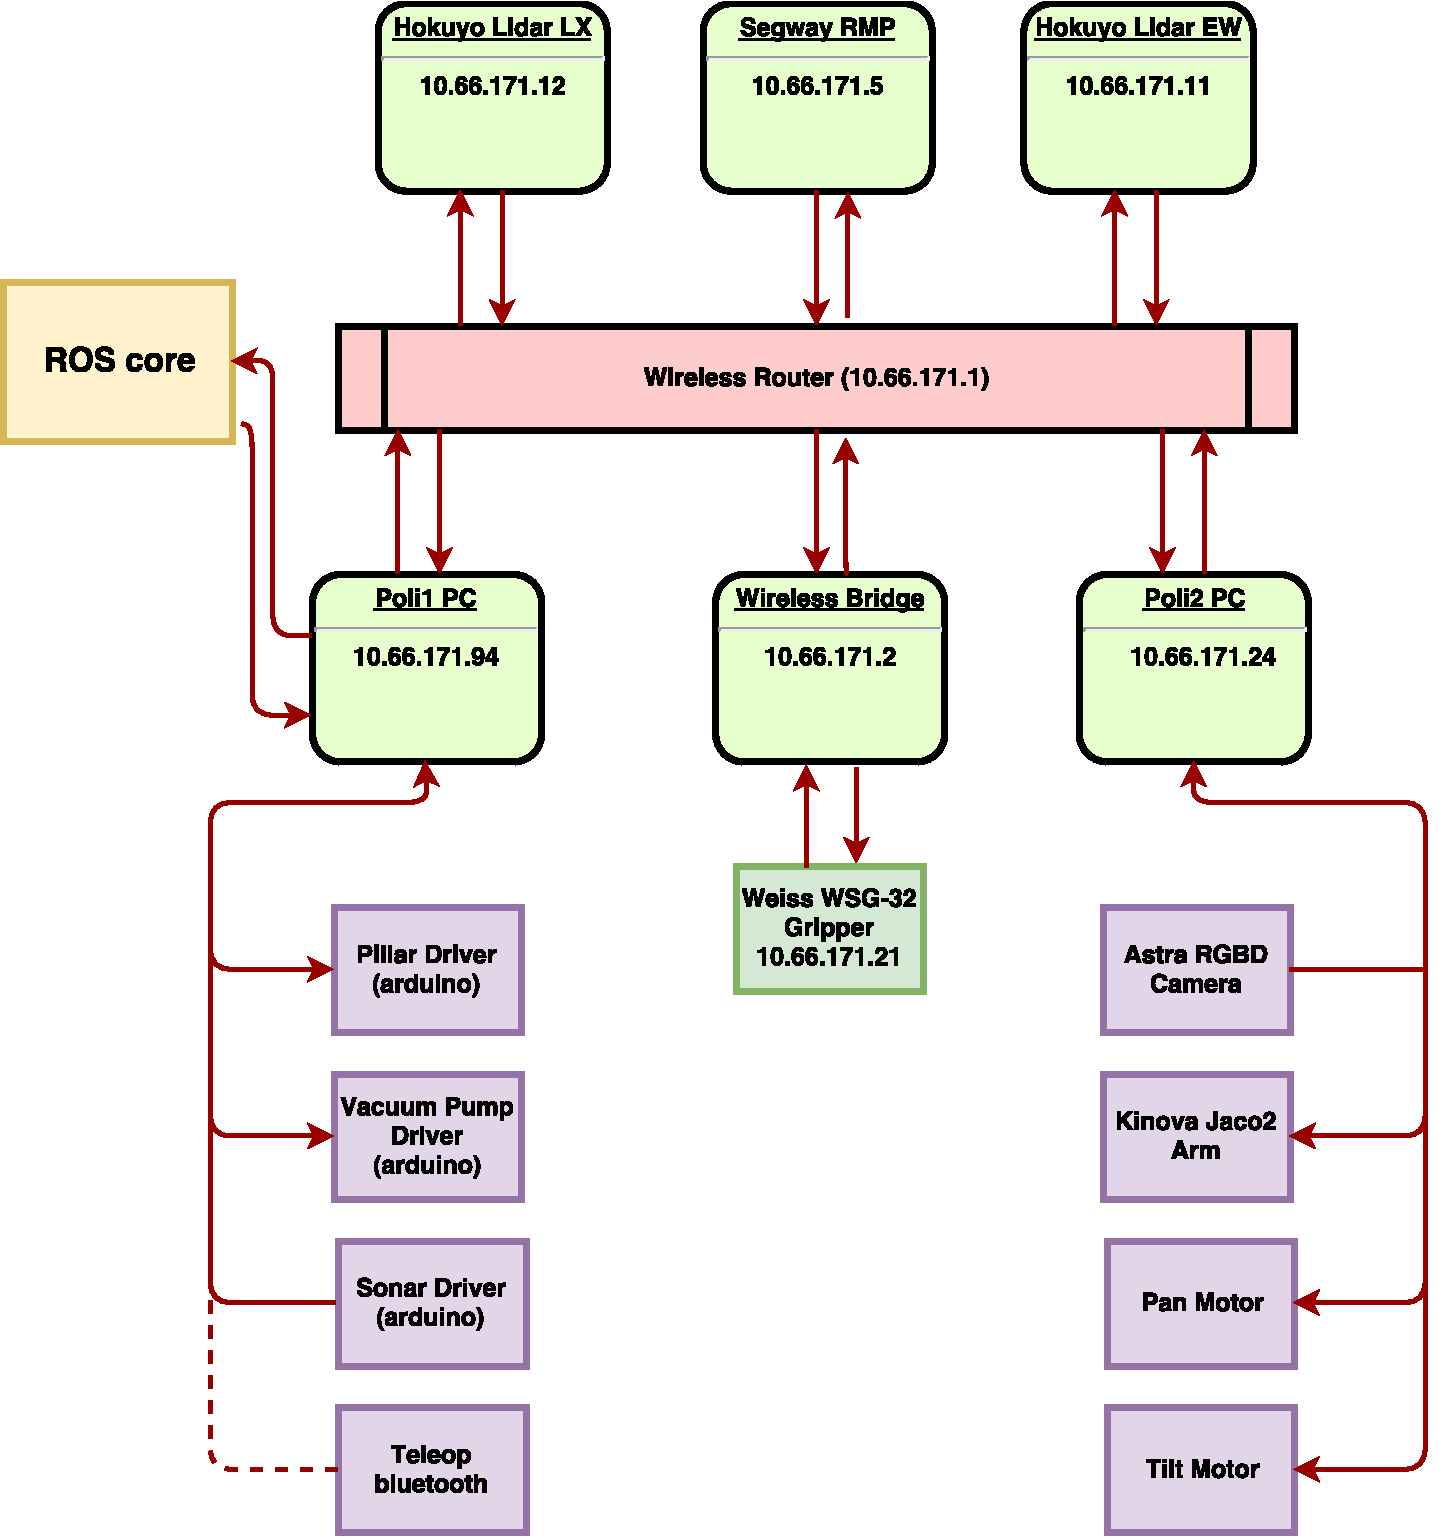
\includegraphics[width=425px]{figures/network_diagram_cropped.pdf}
\caption{Network map for the PoliV2 Robot Platform}
\label{fig:network_map}
\end{figure}

\section{Codebase}
At the time of this writing, the codebase depends heavily on forks and branches of existing opensource packages and libraries. 
This section briefly looks at which fork/branch combination is used and why it was made. \\

Note that fork/branch resolution happens automatically through \texttt{wstool} and that this section is for informational purposes only.

\begin{itemize}
   \item segway\_v3 - Stanley Innovation - \texttt{master} : no kinetic release
   \item wsg\_32\_description - SI-Machines - \texttt{master} : no kinetic release
   \item ira\_laser\_tools - iralabdisco - \texttt{master} : no kinetic release
   \item kinova\_ros - GT-RAIL - \texttt{7dof\_kinetic} : no kinetic release + 7dof changes. Follows \texttt{7dof} branch of same fork.
   \item wsg50-ros-pkg - SI-Machines - \texttt{kinetic-devel} : no kinetic release; URDF and driver bug fixes.
   \item epos\_hardware - RIVeR-Labs - \texttt{kinetic-devel} : no kinetic release
   \item dynamixel-workbench - ROBOTIS-GIT - \texttt{master} : Kinetic release is broken
   \item dynamixel-workbench-msgs - ROBOTIS-GIT - \texttt{master} : Kinetic release is broken
\end{itemize}

\subsection{Microcontroller development}
All microcontroller components are arduino IDE compatible. 
All files used to flash onto the particular arduino can be found in \href{https://github.com/si-machines/poli2/tree/master/poli_launch/scripts/arduino}{\texttt{scripts/arduino/}} folder of the \texttt{poli\_launch} package. \\

A guide on how to do development and flash to Arduinos is available at the github wiki: \href{https://github.com/si-machines/poli2/wiki/Arduino-Development}{https://github.com/si-machines/poli2/wiki/Arduino-Development}. \\

Note that the Arduino devices names are given in Figure \ref{fig:network_map}. These device names are definite for the first Poli2 robot, but may change on subsequent robots depending on how device names are assigned.



